\documentclass{article}

\usepackage{times}
\usepackage{graphicx}
\usepackage{subfigure}
\usepackage{natbib}
\usepackage{algorithm}
\usepackage{algorithmic}
\usepackage{lipsum}
\usepackage{todonotes,tikz}
\usepackage{cite}
\usepackage{natbib}


\usetikzlibrary{bayesnet}
\usepackage{jchen2}
\usepackage[accepted]{icml2017}
\icmltitlerunning{Project Title}

\begin{document}

\twocolumn[
\icmltitle{Project Title}
\begin{icmlauthorlist}
  \icmlauthor{Jiafeng Chen}{}
\icmlauthor{Yufeng Ling}{}
\icmlauthor{Francisco Rivera}{}
\end{icmlauthorlist}

\vskip 0.3in
]

\begin{abstract}
  \begin{itemize}
  \item This document describes the expected style, structure, and rough proportions for your final project write-up.
  \item While you are free to break from this structure, consider it a strong prior for our expectations of the final report.
\item Length is a hard constraint. You are only allowed max \textbf{8 pages} in this format. While you can include supplementary material, it will not be factored into the grading process. It is your responsibility to convey the main contributions of the work in the length given.
  \end{itemize}



\end{abstract}

\section{Introduction}
\label{sec:introduction}

Example Structure:
\begin{itemize}
\item What is the problem of interest and what (high-level) are the current best methods for solving it?
\item How do you plan to improve/understand/modify this or related methods?
\item Preview your research process, list the contributions you made, and summarize your experimental findings.
\end{itemize}


\section{Background}
Example Structure:
\begin{itemize}
\item What information does a non-expert need to know about the problem domain?
\item What data exists for this problem?
\item What are the challenges/opportunities inherent to the data? (High dimensional, sparse, missing data, noise, structure, discrete/continuous, etc?)
\end{itemize}



\section{Related Work}

Example Structure:
\begin{itemize}
\item What 3-5 papers have been published in this space?
\item How do these  differ from your approach?
\item What data or methodologies do each of these works use?
\item How do you plan to compare to these methods?
\end{itemize}




\section{Model}

We represent a city's road network with a connected graph $G = (V,E)$. Assume that each vertex $i \in V$ is associated with a weight $w_i$, representing the cost of traversing vertex $i$. A trip is represented by a path in $G$, and the distribution of the trip's duration depends on the weights $w_i$ of vertices included in the path. Note that the choice of the path can in general depend on the collection of weights $\bm W$. In full generality, the model is represented by Figure~\ref{fig:dgm}, where trips in the data are indexed by $(k)$, $T\uppr{k}$ is the observed trip duration, and $Z\uppr{k}$ is the path taken by trip $k$, a latent variable. Our primary interest is to perform inference on $\bm W$, so as to learn the levels of congestion associated with each vertex in $G$.

\begin{figure}[h]
  \centering
  \caption{Representation of model as a directed graph}
  \label{fig:dgm}
  \vspace{1em}
  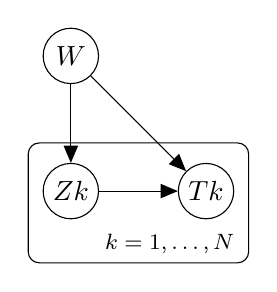
\begin{tikzpicture}
    \node[latent] (W) {$\bm W$};
    \node[latent, below=of W] (Z) {$Z\uppr{k}$};
    \node[latent, right=of Z] (T) {$T\uppr{k}$};
    \edge{W} {Z};
    \edge{W, Z} {T};
    \plate[inner sep=0.5em, yshift=0.2em] {ZT} {(Z) (T)} {$k=1,\ldots,N$} ;
  \end{tikzpicture}
\end{figure}

\subsection{Parameterization}

In principle, in our application to the New York City taxi data, we may take $G$ to be a graph representing the exact road network in New York City, where each vertex is a \emph{road segment} and the directed edge $(i,j) \in E$ if one can drive directly onto road segment $j$ from road segment $i$; such a parameterization allows $w_i$ to be directly interpretable as a measure of congestion on road segment $i$. However, such a detailed construction presents serious computational challenges when training on a large dataset, since solving path-finding problems and computing minimal paths are nontrivially expensive.\footnote{Manhattan has on the order of $10^4$ road segments, and the dataset contains the order of $10^7$ trips for January 2009 alone.} 

To avoid these challenges, we parameterize $G$ as an undirected rectangular grid. Despite not being able to pinpoint weights $w_i$ to congestion of specific road segments, we are nonetheless able to interpret the weights $w_i$ as representative of congestion on a small patch of land. We may now represent a path $Z\uppr{k}$ as a set of indices $i$ of grid points traversed by the path. In full generality, there are an infinite number of paths connecting any two points $i,j$ on the grid, but the vast majority of these paths are not sensible. Thus we restrict the set of possible paths for trip $k$ to a \emph{set of reasonable paths} $\bm Z\uppr{k}$, where each path in $\bm Z\uppr{k}$ travels strictly in the direction of the destination. For instance, if the destination of $j$ is to the northeast of the starting location $i$, then the set of reasonable paths $\bm Z$ are the set of paths that only involve northward or eastward movements (e.g.~Figure~\ref{fig:reasonable} shows a reasonable path from $(0,0)$ to $(2,1)$). Such a parameterization is more general than many in the literature; \citet{zhan2013urban}, for instance, uses the $K$-shortest path algorithm and considers the shortest 20 paths as a set of reasonable paths.

\begin{figure}[h]
\centering
\caption{An example of a reasonable path}
\vspace{1em}

\label{fig:reasonable}
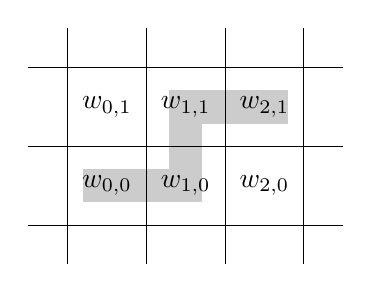
\begin{tikzpicture}
\draw (-0.5,0) -- (3.5,0);
\draw (-0.5,1) -- (3.5,1);
\draw (-0.5,2) -- (3.5,2);

\draw (0,-0.5) -- (0,2.5);
\draw (1,-0.5) -- (1,2.5);
\draw (2,-0.5) -- (2,2.5);
\draw (3,-0.5) -- (3,2.5);

\foreach \y in {0,1}
{
  \foreach \x in {0,...,2}
  {
    \node at (\x+.5,\y+.5) {$w_{\x,\y}$};
  }
}

\draw[line width = 12pt, opacity=.2] (0.2,.5) -- (1.5,.5) -- (1.5,1.5) -- (2.8,1.5);
\end{tikzpicture}
\end{figure} 

We parameterize the conditional distribution of $T\uppr{k}$ as Normal, in the following reformulation of the directed graphical model: \begin{align*}
\bm W &\sim p(\bm W) \\
Z\uppr{k} &\sim p(Z\uppr{k} | \bm W) \\
T\uppr{k} | \bm W, Z\uppr{k} &\sim \Norm\pr{\sum_{i\in Z\uppr{k}} w_i, \sigma^2},
\end{align*}
where $p(Z\uppr{k} | \bm W)$ is a distribution over $\bm Z^{\uppr{k}}$. We consider two different ways to parameterize $p(Z\uppr{k} | \bm W)$: softmax regression and uniform. In the \emph{softmax regression} model, a type of generalized linear model for discrete choice problems \cite{mcfadden1973conditional}, we parameterize the route choice such that \[
p(Z\uppr{k}|\bm W) \propto \exp\pr{-\sum_{i\in Z\uppr{k}}w_i},
\]
in order to encode the fact that drivers avoid routes that take a long period of time. In the \emph{uniform} model, we simply assume that route choice is independent and uniform on the set of reasonable paths: \[
p(Z\uppr{k}|\bm W) \propto 1.
\]
The uniform model trades off realism in modeling for improvement in computation and training, as we see in Section~\ref{sec:inference}.

In our application to the Manhattan dataset, we perform MLE inference, or, equivalently, MAP inference with $p(\bm W) \propto 1$. In principle, it is not difficult to parameterize the prior of $\bm W$ as an undirected graphical model, since we need only to supply edge and unary potentials. For instance, to impose a correlated prior on $\bm W$, as suggested by some \cite{hunter2009path}, we simply penalize large differences in neighboring weights in the edge potential, effectively assuming a prior model that is similar to a continuous version of the Ising model. 



{
\color{gray}
Example Structure:

\begin{itemize}
\item What is the formal definition of your problem?
\item What is the precise mathematical model you are using to represent it? In almost all cases this will use the probabilistic language from class, e.g.
  \begin{equation}
  z \sim {\cal N}(0, \sigma^2)\label{eq:1}
\end{equation}
But it may also be a neural network, or a non-probabilistic loss,
\[ h_t \gets \mathrm{RNN}(x_{t}, h_{t-1} )\]

This is also a good place to reference a diagram such as Figure~\ref{fig:diagram}.

\item What are the parameters or latent variables of this model that you plan on estimating or inferring? Be explicit. How many are there? Which are you assuming are given? How do these relate to the original problem description?
\end{itemize}
}





% \begin{figure}
%   \centering
%   \missingfigure[figheight=8cm]{}
%   \caption{\label{fig:diagram} This is a good place to include a diagram showing how your model works. Examples include a graphical model or a neural network block diagram.}
% \end{figure}


\section{Inference (or Training)}
\label{sec:inference}
We perform maximum likelihood inference, maximizing \[
\max_{\bm W} \log p(\{T\uppr{k}\}_{k=1}^N|\bm W) = \max_{\bm W} \sum_{k=1}^N \log p(T\uppr{k} | \bm W).
\]
The log-likelihood is 
\begin{align*}
&\log p (T\uppr{k} | \bm W) \\
=& \log\pr{\sum_{Z\uppr{k} \in \bm Z\uppr{k}} p(T\uppr{k}|Z\uppr{k},\bm W)p(Z\uppr{k}|\bm W)} \\
=& \log\pr{\E_{Z\uppr{k}}\bk{p(T\uppr{k}|Z\uppr{k},\bm W)}}.
\end{align*}
The expectation is a sum of the size $|\bm Z\uppr{k}|,$ which, for an $m\times n$ trip\footnote{By an $m\times n$ trip, we mean a trip with east-west distance $n$ and north-south distance $m$}, is of $\binom{m+n}{n} \approx \frac{(n+m)^n}{n^n}e^n$ terms. Computing this expectation is the main inference challenge of our project.

\subsection{Inference in the uniform model}

By assuming the uniform model $p(Z|\bm W) \propto 1$, we gain the ability to work with an expectation over $\bm W$ instead of an expectation over $\bm Z$, since the probability that a particular weight is included in a path is readily computable from elementary combinatorics. We maximize an approximate lower bound of the log-likelihood by applications of Jensen's inequality: \begin{align*}
\ell(\bm W) &= \log\pr{\E_{Z\uppr{k}}\bk{p(T\uppr{k}|Z\uppr{k},\bm W)}} \\
&\ge -\frac{1}{2\sigma^2}\pr{T\uppr{k} - \E\bk{\sum_{i\in Z\uppr{k}} w_i}}^2 + \text{const.} \tag{$*$} \\
&= -\frac{1}{2\sigma^2}\pr{T\uppr{k} - \sum_{i} w_i\pi_i}^2 + \text{const.},
\end{align*}
where $\pi_i$ is the marginal probability of node $i$ being included in a uniform route.\footnote{$\pi_i$ can be computed analytically. Suppose the source and destination of the trip are $(n,m)$ apart and vertex $i$ is $(a,b)$ away from the source. Then, by elementary combinatorics, \[\pi_i = \frac{\binom{a+b}{a}\binom{n+m-a-b}{n-a}}{\binom{n+m}{n}}\]} Note that $(*)$ is only a lower bound if $T\uppr{k} - \sum w_i$ is small compared to $\sigma^2$, since for small values of $T\uppr{k} - \sum w_i$ relative to $\sigma$, the Normal density is concave, and the inequality follows by Jensen's inequality. We indeed make this assumption. By assuming a structure of $Z|\bm W$, we gain a great deal of convenience in computation, effectively reducing a sum of $\binom{n+m}{n}$ terms to a sum of merely $nm$ terms. 
 
 
\subsection{Inference in the softmax regression model}




{\color{gray}
\begin{itemize}
\item How do you plan on training your parameters / inferring the
  states of your latent variables (MLE / MAP / Backprop / VI / EM / BP / ...)

\item What are the assumptions implicit in this technique? Is it an approximation or exact? If it is an approximation what bound does it optimize?

\item What is the explicit method / algorithm that you derive for learning these parameters?
\end{itemize}



\begin{algorithm}
  \begin{algorithmic}
    \STATE{}
  \end{algorithmic}
  \caption{Your Pseudocode}
\end{algorithm}
}



\section{Methods}

\begin{itemize}
\item What are the exact details of the dataset that you used? (Number of data points / standard or non-standard / synthetic or real / exact form of the data)

\item What are the exact details of the features you computed?


\item How did you train or run inference? (Optimization method / hyperparameter settings / amount of time ran / what did you implement versus borrow / how were baselines computed).

\item What are the exact details of the metric used?
\end{itemize}



\section{Results}

\begin{itemize}
\item What were the results comparing previous work / baseline systems / your systems on the main task?
\item What were the secondary results comparing the variants of your system?
\item This section should be fact based and relatively dry. What happened, what was significant?
\end{itemize}

\begin{table*}
  \centering
  \missingfigure{}
  \caption{This is usually a table. Tables with numbers are generally easier to read than graphs, so prefer when possible.}
  \label{fig:mainres}
\end{table*}


% \begin{table}
%   \centering
%   \missingfigure[figheight=5cm]{}
%   \caption{Secondary table or figure in results section.}
%   \label{fig:mainres}
% \end{table}



\section{Discussion}



\begin{itemize}
\item What conclusions can you draw from the results section?
\item Is there further analysis you can do into the results of the system? Here is a good place to include visualizations, graphs, qualitative analysis of your results.

\item  What questions remain open? What did you think might work, but did not?
\end{itemize}



% \begin{figure}
%   \centering
%   \missingfigure{}
%   \missingfigure{}
%   \missingfigure{}
%   \caption{Visualizations of the internals of the system.}
% \end{figure}

\section{Conclusion}

\begin{itemize}
\item What happened?
\item What next?
\end{itemize}



% \section*{Acknowledgements}

% \textbf{Do not} include acknowledgements in the initial version of
% the paper submitted for blind review.

% If a paper is accepted, the final camera-ready version can (and
% probably should) include acknowledgements. In this case, please
% place such acknowledgements in an unnumbered section at the
% end of the paper. Typically, this will include thanks to reviewers
% who gave useful comments, to colleagues who contributed to the ideas,
% and to funding agencies and corporate sponsors that provided financial
% support.


\bibliography{biblio.bib}
\bibliographystyle{icml2017}

\end{document}
